\section{Memory Map}
\label{sec:mem_map}

The memory map of the system, as seen by picoVersat programs, is given in
Table~\ref{tab:memmap}.

\begin{table}[!htbp]
  \centering
    \begin{tabular}{|p{3cm}|c|c|c|p{4cm}|}
    \hline 
    {\bf Mnemonic} & {\bf Address} & {\bf Read/Write} & {\bf Read Latency} & {\bf Description} \\
    \hline \hline 
     REGF\_BASE & 0x800 & Read+Write & 0 & Register file peripheral. \\
    \hline
     CPRT\_BASE & 0x812 & Write only & NA & Debug printer periheral. \\
    \hline
     EXT\_BASE & 0x820 & Write only & NA & External interface. \\
    \hline
     DISPLAY0 & 0x820 & Read+Write & 0 & Display0 peripheral. \\ 
    \hline
     DISPLAY1 & 0x822 & Read only & 0 & Display1 peripheral. \\
    \hline
     DISPLAY2 & 0x824 & Read only & 0 & Display2 peripheral. \\
    \hline
     DISPLAY3 & 0x826 & Write only & 0 & Display3 peripheral. \\
    \hline
     LED\_BASE & 0x828 & Write only & 0 & LED peripheral. \\
    \hline
     SWITCH\_BASE & 0x82A & Write only & 0 & SWITCH peripheral. \\
    \hline
     BUTTON\_BASE & 0x82C & Write only & 0 & BUTTON peripheral. \\
    \hline
     LFSR\_BASE & 0x82E & Read only & 1 & LFSR peripheral. \\
    \hline
     PROG\_BASE & 0x0 & Read+Write & 1 & User programs and data. \\
    \hline
    \end{tabular}
  \caption{Memory map base addresses}
  \label{tab:memmap}
\end{table}

\clearpage
\section{Program Description}
\label{sec:pgrm}
The state diagram of the Fig.~\ref{fig:state}, it's the proposal system to implement, 
this diagram is intend to give an abstract description of the behavior of tthe system that 
will be running in the PicoVersat processor. This behavior is represented as a series of events 
that occur in the three states, and by this events the program will flow the schematic doing the 
value of the events.

\noindent
The idle state has the main objective of reset all the important variables of the system, after reseting the value of each led, score and level. 
The system waits until the user pressed the condition of start to initiate the game and call the show state.

\noindent
The show state is where a new level is generated, a new random sequence is shown in the led's.
As the level increases the time between each led blinking increases too. 

\noindent
The game state have the responsibility of checking each move and increment the respective score and level. This state will show the value of each level and score. After the player win the game or loose the system will return to the idle mode showing a message that the 
player have won the game.

\begin{figure}[!htbp]
    \centerline{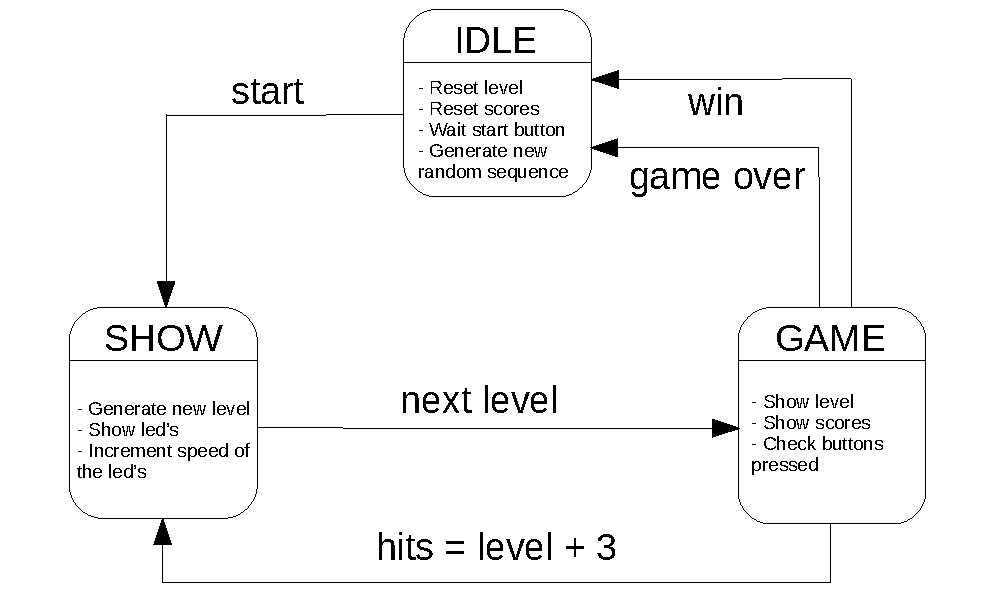
\includegraphics[width=\textwidth]{state}}
    \vspace{0cm}\caption{State diagram}
    \label{fig:state}
\end{figure}
